\documentclass[tikz]{standalone}

\usetikzlibrary{patterns}

\begin{document}
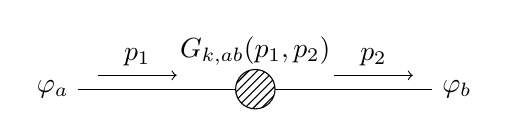
\begin{tikzpicture}
  \draw (-2.25,0) node[left] {$\varphi_a$} -- (2.25,0) node[right] {$\varphi_b$};
  \draw[->,yshift=5pt] (-2,0) -- (-1,0) node[midway,above] {$p_1$};
  \draw[->,yshift=5pt] (1,0) -- (2,0) node[midway,above] {$p_2$};
  \draw[fill=white,postaction={pattern=north east lines}] (0,0) circle (0.25) node[above=5pt] {$G_{k,ab}(p_1,p_2)$};
\end{tikzpicture}
\end{document}
